\section{EODP-TS-L1B. Level-1B processing}
\label{sec:l1b}

\subsection{Objective}
The test validates the L1B module.
The L1B converts the digital numbers of the ISM back into TOA radiances in two steps \cite{atbd}.
\begin{itemize}
\item Equalization. It removes the offset and the gain of each pixel: $DN_{eq} = (DN - eq_{add}) / eq_{mult}$.
\item Restoration. It applies the absolute radiometric gain of the band: $L_{L1B} = DN_{eq} \cdot g$.
\end{itemize}

\subsection{Inputs and configuration}
The input is the ISM output in \texttt{EODP\_TER\_2021/EODP-TS-L1B/input}.
It contains \texttt{ism\_toa} in DN and \texttt{ism\_toa\_isrf}, the radiance before the instrument effects.
The equalization factors are the files \texttt{eq\_add} and \texttt{eq\_mult} of the auxiliary folder. They have one value per ACT pixel.
The absolute gains are 0.0921, 0.0679, 0.0522 and 0.0478 mW/m$^2$/sr/DN for the four bands.

\subsection{Execution}
The script \texttt{harness/EODP-TS-L1B/test\_l1b.py} runs the L1B twice.
The first run has \texttt{do\_equalization = False}. The second run has \texttt{do\_equalization = True}. The second run is the one cross-validated.

\subsection{Results}

\subsubsection{Cross-validation}
Table~\ref{tab:l1b_crossval} shows the comparison of the equalized DN and the L1B radiances with the reference.
All the files are identical to the reference.

\begin{longtable}{lccccc}
\caption{L1B cross-validation with equalization. Maximum relative difference [\%] per band.}\label{tab:l1b_crossval}\\
\toprule
File & VNIR-0 & VNIR-1 & VNIR-2 & VNIR-3 & Result \\
\midrule
\endfirsthead
\toprule
File & VNIR-0 & VNIR-1 & VNIR-2 & VNIR-3 & Result \\
\midrule
\endhead
\texttt{l1b\_toa\_eq\_} & $0$ & $0$ & $0$ & $0$ & Pass \\
\texttt{l1b\_toa\_} & $0$ & $0$ & $0$ & $0$ & Pass \\
\bottomrule
\end{longtable}


\subsubsection{Calibration plot}
Figure~\ref{fig:l1b_calibration} shows the central ALT line of three images.
The black line is the TOA after the ISRF. It is the radiance that enters the instrument and it is taken as the truth.
The red line is the L1B without equalization. The blue line is the L1B with equalization.

\begin{figure}[H]
\centering
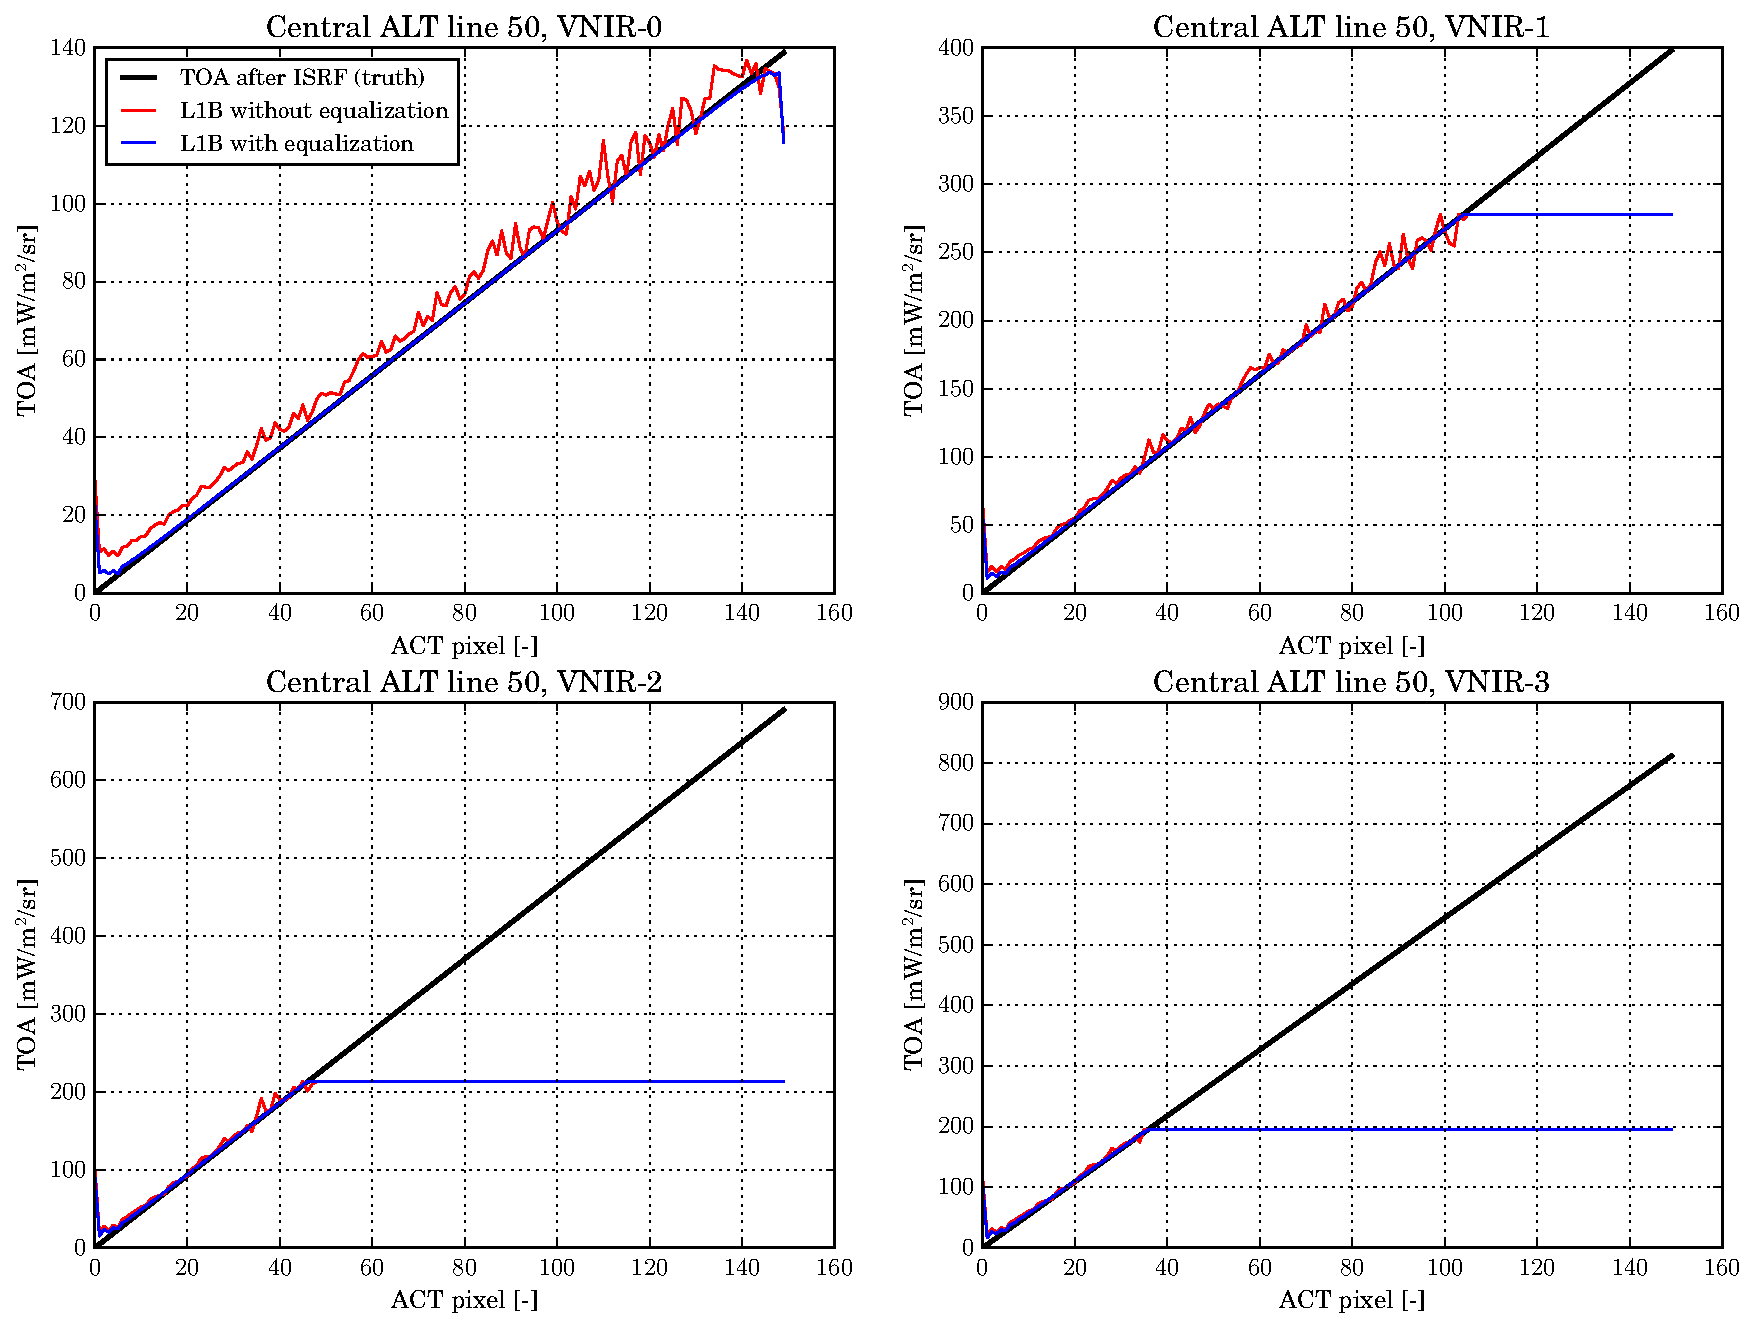
\includegraphics[width=\textwidth]{l1b_calibration}
\caption{L1B. TOA after the ISRF, L1B without equalization and L1B with equalization. Central ALT line.}
\label{fig:l1b_calibration}
\end{figure}

Without equalization the L1B shows the stripes of the PRNU and the DSNU. It is also shifted above the truth because the dark signal adds a positive offset. The shift is clear in VNIR-0, where the signal is low.
With equalization the stripes and the offset disappear and the L1B follows the truth.
Two differences remain.
The first and last columns differ because of the MTF edge effect of the ISM.
In VNIR-1, VNIR-2 and VNIR-3 the L1B becomes flat from a certain column. The L1B is ``blocked'' at a constant value.
This happens because the ISM saturated these pixels at the FWC and at 4095~DN (Section~\ref{sec:ism}). The information above saturation is lost and the L1B cannot recover it.
The flat level is the radiance that corresponds to 4095~DN after the equalization and the gain.

Table~\ref{tab:l1b_errors} gives the median relative error with respect to the truth.
Saturated pixels and the two columns of each border are excluded.
The median is used because the first columns have a radiance close to zero, where any small difference gives a large relative error.
The equalization reduces the error in all the bands.

\begin{table}[H]
\centering
\caption{L1B median relative error with respect to the TOA after the ISRF, and fraction of saturated pixels.}
\label{tab:l1b_errors}
\begin{tabular}{lccc}
\toprule
Band & Error without eq. [\%] & Error with eq. [\%] & Saturated pixels [\%] \\
\midrule
VNIR-0 & 7.494 & 0.233 & 0.0 \\
VNIR-1 & 4.116 & 0.166 & 30.7 \\
VNIR-2 & 4.216 & 0.946 & 68.7 \\
VNIR-3 & 5.047 & 1.655 & 76.7 \\
\bottomrule
\end{tabular}

\end{table}

\subsection{Theoretical question. What is calibration?}
Calibration is the process that finds the parameters which relate the instrument output to the physical quantity observed.
The instrument does not measure radiance. It produces digital numbers. Each pixel has its own response, with an offset from the dark signal and a gain from the PRNU.
The calibration has two parts.
\begin{itemize}
\item Relative calibration. It finds the offset and the gain of each pixel, so that all the pixels give the same output for the same input. These are the equalization factors $eq_{add}$ and $eq_{mult}$. The offset is measured with dark images, without illumination. The gain is measured with a uniform scene.
\item Absolute calibration. It finds the gain $g$ that converts the equalized DN into radiance. It is measured with a source of known radiance, such as an integrating sphere on ground or the Sun with a diffuser in flight.
\end{itemize}
The calibration parameters are measured in the calibration campaigns and stored in a characterisation database.
The L1B processing does not compute them. It only applies them.
Figure~\ref{fig:l1b_calibration} shows the effect. Without the relative calibration the image has stripes and an offset. With it the L1B recovers the input radiance up to the saturation level.

\subsection{Conclusion}
The L1B outputs with equalization match the reference with a relative difference of zero.
The equalization removes the PRNU and DSNU stripes.
\textbf{EODP-TS-L1B: PASS.}
